\chapter{Resultados}
\label{c_resultados}

% Como crianças de 4 a 6 anos interagem com uma interface de programação focada em permitir visualizar os passos e a execução de um algoritmo? 
% Descrever como as crianças interagem com a interface de realidade aumentada

O \autoref{quadro:equipes} apresenta as equipes que participaram dos experimentos. As equipes 1 e 2 são da turma de 5 a 6 anos, e as demais são das turmas de 4 a 5 anos. O tempo de participação de cada equipe variou entre 13 e 35 minutos, devido a casos de não finalização da atividade. O tempo de 35 minutos, porém, foi suficiente para concluir todas as etapas, desde a ambientação até os problemas de depuração. Outro fator de influência na duração da atividade foi a troca de participantes, que entraram na brincadeira depois do início ou saíram antes do fim. Nesses casos, a equipe da criança é o grupo onde ela permaneceu por mais tempo. A criança C10 também integrou duas equipes para C14 não brincar individualmente.

\begin{quadro}[!h]
    \caption{Equipes.}
    \label{quadro:equipes}
    \centering
    {
        \begin{footnotesize}
        {\renewcommand{\arraystretch}{1.2}
        \begin{tabular}{|l|l|l|l|} 
            \hline
            \textbf{ Equipe/Tempo }                                  & \textbf{Criança } & \textbf{Idade} & \textbf{Sexo} \\ 
            \hline
            
            \multirow{2}{*}{Equipe 1. 35min}                & C1               & 5:10                         & Masculino \\ 
            \cline{2-4}
                                                                                        & C2               & 5:7                          & Masculino \\ 
            \hline
            \multirow{2}{*}{Equipe 2. 35min}                & C3               & 5:10                         &  Feminino \\ 
            \cline{2-4}
            \multicolumn{1}{|c|}{}                                      & C4               & 5:11                         &  Feminino \\ 
            \cline{2-4}
            \multicolumn{1}{|c|}{}                                      & C5               & 6:0                          & Feminino \\ 
            \hline
            
            \multirow{2}{*}{Equipe 3. 24min}                & C6               & 4:10                         & Masculino \\ 
            \cline{2-4}
                                                                                        & C7               & 3:11                         & Masculino  \\ 
            \hline
            Equipe 4. 13min                                                 & C8               & 4:3                          & Masculino \\ 
            \hline
            \multirow{3}{*}{Equipe 5. 23min}                & C9               & 4:7                          & Masculino  \\ 
            \cline{2-4}
                                                                                    & C10              & 4:8                          & Masculino   \\ 
            \cline{2-4}
                                                                                    & C11              & 4:8                          & Masculino   \\ 
            \hline
            \multirow{2}{*}{Equipe 6. 19min}                & C12              & 4:2                          &  Feminino \\ 
            \cline{2-4}
                                                                                     & C13              & 4:3                          &  Feminino \\ 
            \hline
            \multirow{2}{*}{Equipe 7. 10min}                & C14              & 4:10                         &  Feminino \\ 
            \cline{2-4}
                                                                                        & C10              & 4:8                          &  Feminino \\ 
            \hline
            \multirow{2}{*}{Equipe 8. 30min}                & C15              & 4:7                          & Masculino \\ 
            \cline{2-4}
                                                                                        & C16              & 4:5                          &  Feminino \\ 
            \hline
            \multirow{2}{*}{Equipe 9. 20min}                & C17              & 4:3                            &  Feminino \\ 
            \cline{2-4}
                                                                                        & C18              & 4:5                            & Masculino \\ 
            \hline
            \multirow{2}{*}{Equipe 10. 22min}               & C19              & 4:4                            & Masculino \\ 
            \cline{2-4}
                                                                                        & C20              & 4:6                            & Masculino  \\
            \hline
            \end{tabular}
        }
        \end{footnotesize}
    }
\end{quadro}

\section{Análise indutiva}
Essa seção apresenta as observações a respeito de como as crianças perceberam e interagiram com os blocos de código tangíveis, e em seguida comenta as suas percepções sobre os elementos de realidade aumentada. 

\subsection{Interação com os blocos}

Após as etapas de seleção e ambientação, as crianças iniciaram o reconhecimento dos blocos. O pesquisador mostrou um bloco por vez, selecionado aleatoriamente, para as crianças dizerem seu significado. Essa etapa é importante, pois a programação e a depuração dos algoritmos dependem de compreender o significado dos blocos. 

De modo geral, as crianças entenderam as direções dos blocos, e demonstraram isso principalmente por gestos com as mãos. O principal erro foi confundir as setas de “frente” e “trás” com “cima” e “baixo”. As respostas gestuais indicaram mais erros de vocabulário do que de interpretação. Em 9 momentos as crianças usaram os termos “cima” ou “baixo”, mas apontando para “frente” ou “trás”, e apenas 1 criança realmente entendeu essas setas como sinais verticais. Para os blocos de “esquerda” e “direita”, as crianças usaram o termo “pro lado”, enquanto apontavam para a direção correta (\autoref{quadro:falas_simbolos}).

A associação dos blocos com os botões do RoPE também ocorreu naturalmente, sem a solicitação do pesquisador. Ao perceber que a similaridade de cores entre os blocos e os botões, C1 e C2, e também C10 e C11, apontaram para os botões e aproximaram os blocos dos mesmos. Um caso diverso apareceu na Equipe 2, em que as crianças C4, C5 e C6 ignoraram os blocos e mantiveram atenção apenas nos botões do brinquedo.

Essas interações também evidenciaram a necessidade de modificar o design dos blocos. Na segunda fala do \autoref{quadro:falas_simbolos}, C4 aponta o círculo da marca fiducial do bloco Frente e entende que o brinquedo está “rodando”. A criança entendeu o bloco posteriormente, mas sua primeira percepção indica que a marca fiducial chamou sua atenção. Portanto, o ideal seria eliminar a marca, pois ela não possui um significado útil para a criança. Em outro caso, C17 falou sobre o bloco Frente: \fala{Ele “tá” secando as mãos}. Uma possível origem desta resposta seria entender os quatro riscos desenhados no bloco Frente como símbolo de "vento". Essa criança compreendeu o significado correto posteriormente, mas sua fala indica que a imaginação fértil da criança, associada a detalhes de design, a fizeram obter uma conclusão inesperada.

\begin{quadro}[htbp]
    \captionquadro{Falas sobre os símbolos dos blocos.}
    \label{quadro:falas_simbolos}
    \begin{footnotesize}
    \begin{longtable}{ | m{.2\textwidth} | m{.7\textwidth} |}
        \hline
        \textbf{Bloco}  & \textbf{Falas e diálogos} \hline
        \endhead
        
        %%%%%%%%%%%%%%%%%%%
    
        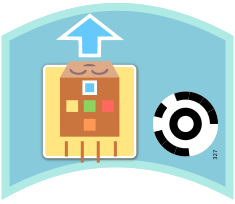
\includegraphics[width=.9\linewidth]{figs/blocks/frente.png} &
    
        \makecell{
            \falapessoa{C2}{Ele tá botando... o sistema dele pra cima.} \\
            \falapessoa{C1}{Ele tá olhando pra cima.} \\
            \\
            \falapessoa{C4}{Rodando} \gesto{Aponta marca fiducial, que é redonda}\\
            \\
            \falapessoa{C4 e C5}{Pra aquele (lado)} \gesto{apontam para frente} \\
            \falapessoa{C3}{Pra aquele} \gesto{aponta pra cima} \\
            \falapessoa{Pesquisador}{Pra cima?} \gesto{C3 confirma com a cabeça} \\
            \\
            \falapessoa{C10}{Uma flechinha} \\
            \falapessoa{Pesquisador}{Uma flechinha pra onde?} \\
            \falapessoa{C10}{Pra cima} \gesto{aponta pra frente} \\
            \falapessoa{C9}{Tipo daquelas ferramentas} \gesto{aponta brinquedos à frente} \\
            \\
            \falapessoa{Pesquisador}{O que ele tá fazendo aqui nesse desenho?} \\
            \falapessoa{C13}{Dormindo!} \\
            \\
            \falapessoa{C17}{Eu acho que ele tá secando as mãos... Eu acho que ele tá indo pra frente} \\
            \\
            \falapessoa{Pesquisador}{Esse bloquinho ele tá indo pra onde?} \\
            \falapessoa{C15}{Pra pegar a maçã.}
        }

        \\ \hline

        %%%%%%%%%%%%%%%%%%%

        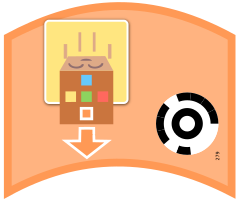
\includegraphics[width=.9\linewidth]{figs/blocks/tras.png} &

        \makecell{
            \falapessoa{C1}{Esse aqui ele tá olhando pra baixo.} \\
            \\
            \falapessoa{C10}{Pra baixo.}  \\
            \falapessoa{C9}{Pra baixo!}  \\
            \falapessoa{Pesquisador}{E onde é pra baixo aqui no robô?} \\
            \falapessoa{C10}{Grama} \gesto{Aponta para o chão}  \\
            \falapessoa{Pesquisador}{Qual é o botão que faz ele ir pra trás?} \\
            \falapessoa{C9}{Aqui} \gesto{aponta botão trás} \\
            \\
            \falapessoa{C17}{Ele tá indo pra trás} \\
            \falapessoa{C5}{Pra baixo.} \\
            \falapessoa{C4}{Esse aqui ele tá olhando pra baixo.} \\
        }

        \\ \hline

        %%%%%%%%%%%%%%%%%%%

        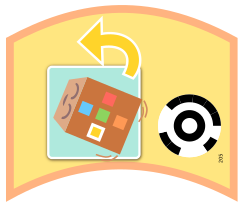
\includegraphics[width=.9\linewidth]{figs/blocks/esquerda.png} &

        \makecell{
            \falapessoa{C2}{Ele tá olhando pra aquele lado.} \gesto{aponta para a esquerda} \\
            \falapessoa{C5}{[tá rodando] pra aquele [lado].} \gesto{gira corpo para a esquerda} \\
            \falapessoa{C10}{Esse aqui ó.} \gesto{aponta para a esquerda}
        }

        \\ \hline

        %%%%%%%%%%%%%%%%%%%

        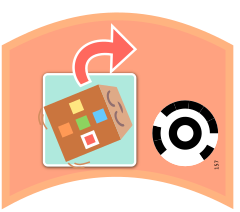
\includegraphics[width=.9\linewidth]{figs/blocks/direita.png} &

        \makecell
        {
            \falapessoa{C2}{Esse aí ele tá olhando pro lado.} \gesto{aponta para a direita} \\
            \falapessoa{C10}{Pro lado.} \gesto{aponta para botão do RoPE} \\
            \\
            \falapessoa{Pesquisador}{Ele tá fazendo alguma coisa?} \\
            \falapessoa{C13}{Tá dormindo! De novo.} \\
        }

        \\ \hline

        %%%%%%%%%%%%%%%%%%%

        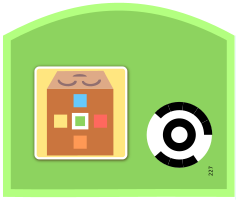
\includegraphics[width=.9\linewidth]{figs/blocks/inicio.png} &

        \makecell{
            \falapessoa{C1}{Esse aqui também [está olhando pra cima].} \\
            \falapessoa{C1}{Esse aqui é pra tirar vários.} \\
        }

        \\ \hline

        %%%%%%%%%%%%%%%%%%%

    \end{longtable}
    \end{footnotesize}
\end{quadro}

\begin{quadro}[!h]
   \begin{table_env}
   \caption{Reconhecimento dos blocos}
    \label{quadro:reconhecimentoblocos}
    \begin{tabular}{@{}l m{.6\textwidth} c@{}}
        \toprule
        Categoria                   & Descrição                                                                  & Frequência \\ \midrule
        "pro lado"                  & Aponta para a direção correta, mesmo não usando as palavras \fala{direita} ou "esquerda"                                           & 5 \\
        "pra cima"                  & Fala ou aponta direção correta, mesmo falando outras palavras              & 4 \\
        Outros                      & Menciona algo não relacionado a movimento                                  & 3 \\
        "pra baixo"                 & Aponta ou fala a direção correta usando outras palavras                    & 2 \\
        Relaciona com o botão       & Aponta botão relacionado                                                   & 2 \\
        Menciona esquerda/direita   & Menciona palavras \fala{esquerda} e \fala{direita} durante reconhecimento dos blocos & 1 \\
        "pra trás"                  & Fala a palavra \fala{trás}                                                     & 1 \\
        Rodando                     & Identifica botão frente ou trás como rodando                               & 1 \\
        Aponta pra cima             & Confunde frente com cima, apontando pra cima                               & 1 \\
        Pro chão                    & Diz que o brinquedo está indo pro chão, sem indicar a direção \fala{trás}       & 1 \\ \nidrule
        Indo pegar a maçã           & Diz que o brinquedo está \fala{Indo pegar a maçã}                               & 1 \\ \bottomrule
        \end{tabular}
   \end{table_env}
   \sourceauthor
\end{quadro}

O \autoref{quadro:reconhecimentoblocos} apresenta exemplos das respostas obtidas. Destaca-se a primeira fala, de C2, que ao analisar o bloco Frente diz: \fala{ele está botando... o sistema dele pra cima}. Provavelmente a criança não sabe o que é um sistema, mas sabe que é algo associado a um robô. A dinâmica da atividade não permitiu investigar, naquele instante, qual o entendimento da criança sobre o tema, mas temas relacionados à computação apareceram posteriormente:

\begin{dialogo}
    \gesto{C2 Clica diversas vezes em todos os botões} \\
    \falapessoa{C1}{Para, senão ele vai \textbf{bugar}!} \\
    \falapessoa{Pesquisador}{Bugar? o que é bugar?} \\
    \falapessoa{C1}{É quando ele faz assim ó} \gesto{C1 e C2 fazem posição de “estátua”.}
\end{dialogo}

Esta criança, portanto, entende que \destaque{bugar} é algo relacionado a travamentos e deve ser evitado. Outras crianças apresentaram outras justificativas quando o robô não se moveu: C14 disse: \fala{Não anda esse robô. Tava dormindo, coitadinho}. O vocabulário "avançado"\ da Equipe 1 não apareceu nas outras equipes.

A Equipe 1, além de compreender o significado dos blocos, iniciou a exploração dos mesmos, relacionando-os uns com os outros. As crianças começaram a encaixar os blocos iguais entre si, formando 4 grupos de blocos (4 Frente, 2 Esquerda, 2 Direita, 2 Trás) (\autoref{fig:relacao_blocos}). O pesquisador questionou o motivo de tal agrupamento, conforme o diálogo a seguir:

\begin{dialogo}
    \gesto{Crianças encaixam os blocos} \\
    \falapessoa{Pesq}{Dá pra montar né? Dá pra encaixar}{01.59} \\
    \gesto{C2 tenta encaixar peças de cores diferentes} \\
    \falapessoa{C1}{Não, esse aqui não pode. Esse aqui não é desse.}{02.06} \\
    \falapessoa{C2}{É um jogo…}{02.08} \\
    \falapessoa{C1}{Esse aqui tá olhando pra baixo.}{02.11} \gesto{segura bloco Trás} \\
    \falapessoa{C1}{Esse aqui vou conectar com esse, e esse conecta com esse}{02.20} \gesto{unindo peças de mesma cor} \\
    \falapessoa{Pesq}{Porque esses assim?}{02.30} \\
    \falapessoa{C1}{Porque tão olhando pro mesmo lado né!}{02.32} \\
    \falapessoa{Pesq}{Ah... e pela cor né}{02.36} \\
    \falapessoa{C1}{Não, porque tão olhando pro mesmo lado!}{02.40} \\
    \falapessoa{Pesq}{Ah... entendi...}{02.40}
\end{dialogo}

A justificativa para tal associação, portanto, foi a posição do brinquedo desenhado, e não cor do bloco. Percebendo a similaridade entre pares de blocos, C1 sugeriu que poderia ser jogado o "Jogo da Memória". O pesquisador e os dois meninos então viraram os blocos com a face para baixo (\autoref{fig:jogo_memoria}), e, cada um por vez, virou duas peças.

\begin{figure}[!htbp]
    \begin{center}
    \begin{subfigure}{.5\textwidth}
        \centering
        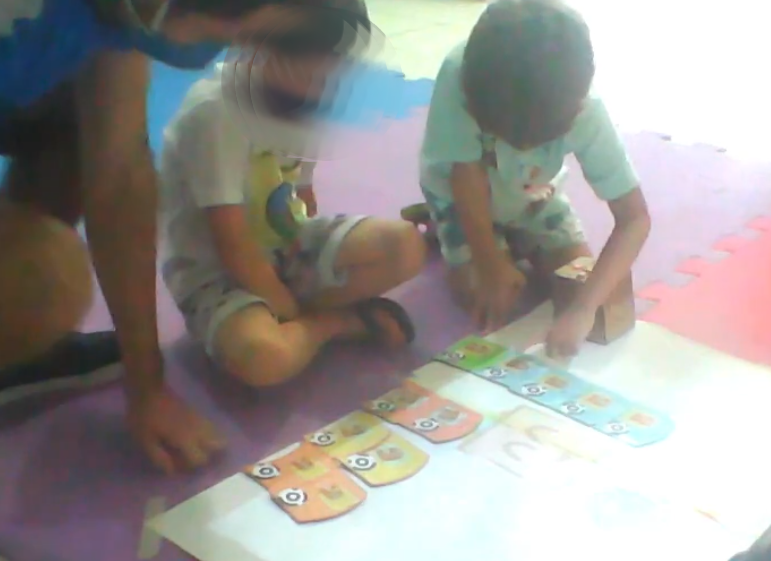
\includegraphics[width=.9\linewidth,fbox]{figs/relacao_blocos.png}
        \caption{Relacionamento entre blocos}
        \label{fig:relacao_blocos}
    \end{subfigure}%
    \begin{subfigure}{.4\textwidth}
        \centering
        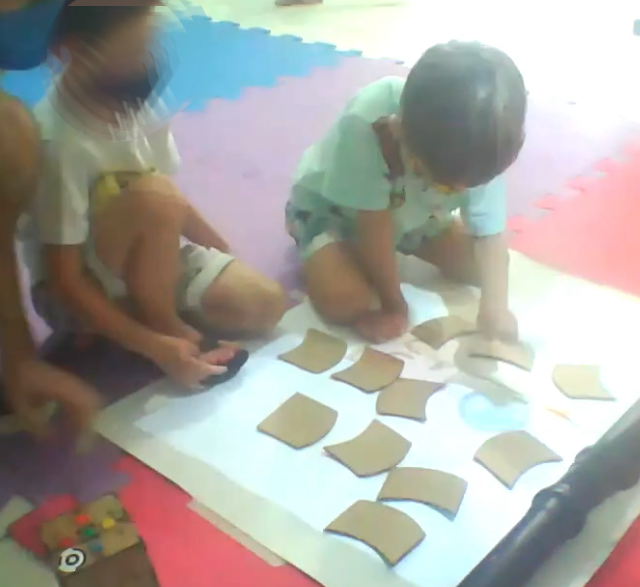
\includegraphics[width=.9\linewidth,fbox]{figs/jogo_memoria.png}
        \caption{Jogo da memória, proposto pela dupla}
        \label{fig:jogo_memoria}
    \end{subfigure}
    \end{center}
    \sourceauthor
    \label{fig:equipe1}
\end{figure}

Outro aspecto de design a ser melhorado apareceu durante o jogo: os blocos Direita e Trás tem cores muito parecidas (tons de vermelho e laranja). Ao procurar blocos iguais, C2 virou um bloco Trás e um bloco Direita e considerou um ponto ganho. C1 alertou o colega ao perceber o engano, e C2 devolveu os blocos. O diálogo revela a interação entre as crianças durante o jogo:

\begin{dialogo}
    \falapessoa{C2}{Agora é minha vez.}\gesto{vira peças vermelha e laranja, e pensa que acertou}{11.57} \\
    \falapessoa{C1}{Errou, é diferente.}{12.00} \\ 
    \falapessoa{Pesq}{É diferente né. Mas é parecido, é parecido.}{12.05}
\end{dialogo}

A mesma situação ocorreu com C8, que selecionou o bloco Trás ao tentar fazer o brinquedo girar à Direita. A Prof\_6 então atuou direcionando a atenção da criança para ela perceber o engano:

\begin{dialogo}
    \falapessoa{Pesq}{Viu que ele foi pra trás? Porque aqui tá o bloquinho laranja. O que ele tem que fazer?} \\
    \falapessoa{C8}{Vermelho!} \\
    \falapessoa{Pesq}{E qual é o bloquinho vermelho?} \\
    \falapessoa{C8}{Esse aqui ó} \gesto{pega o laranja} \\
    \falapessoa{Prof\_6}{Esse é vermelho, tem certeza? Olha bem...} \\
    \falapessoa{Pesq}{Qual é mais vermelho. Esse ou esse?} \gesto{coloca blocos esquerda e trás lado a lado} \\
    \falapessoa{Prof\_6}{Olha a flechinha se é igual.} \\
    \falapessoa{C8}{Vermelho é esse.} \gesto{aponta bloco Direita} \\
\end{dialogo}

Esses dois diálogos demonstram que a interação com os objetos viabilizou conversas entre as crianças e de professor para criança. Nos dois casos uma criança foi alertada por colega ou professor sobre um erro, e pode então desfazê-lo manipulando os blocos de papelão. No primeiro caso a correção do erro consistiu em virar a face dos blocos para baixo, pois não formavam um par do jogo da memória. No segundo caso, a correção consistiu em encaixar outro bloco na sequência de blocos. Isso demonstra que ações similares surgiram tanto na brincadeira sugerida pelas crianças quanto na construção de um algoritmo. São ações naturais, presentes nas brincadeiras, mas que viabilizam o contato com conceitos de computação e \ac{PC}.

% \subsubsection{Associação dos blocos com os botões}

\subsection{Percepções de realidade aumentada}

O diferencial da RoPE AR para outros tipos de interface de programação é a união entre realidade aumentada e blocos tangíveis. Neste sentido, a questão é: como as crianças perceberam e interagiram com a RA?

Para respondê-la, a análise dos vídeos apontou alguns tipos de eventos em que as crianças perceberam os elementos projetados e os relacionaram com objetos reais. Para contar esses eventos, foram considerados gestos, falas e reações de animação ou estranhamento das crianças (\autoref{quadro:percepcao_ra}).

\begin{quadro}[!h]
    \begin{table_env}
    \caption{Eventos de percepção de realidade aumentada}
     \label{quadro:percepcao_ra}
     \begin{tabular}{@{}l m{.5\textwidth} c@{}}
        \toprule
        Categoria                                      & Descrição                                                                             & Frequência \\ \midrule
        Aponta para figura projetada                   & Criança aponta para uma figura projetada                                              & 32 \\
        Percebe que brinquedo "comeu"\ a maçã           & Criança fala ou gesticula indicando que o brinquedo "comeu"\ a maçã                   & 20 \\
        Levanta brinquedo, procurando maçã             & Criança levanta o brinquedo procurando a maçã que desapareceu                         & 13 \\
        Percebe que maçã apareceu                      & Criança aponta para a maçã que acabou de parecer                                      & 10 \\
        Estranha que não comeu maçã                    & Criança estranha quando o brinquedo não come a maçã ao chegar no quadrado dela        & 5 \\
        Percebe destaque do bloco                      & Criança aponta o bloco destacado pelo projetor                                        & 3 \\
        Tenta tocar no objeto virtual                  & Criança coloca a mão sobre a imagem de alguma figura projetada                        & 3 \\
        Coloca bloco sobre a maçã                      & Criança percebe a localização da figura projetada e coloca um objeto físico sobre ela & 2 \\
        Percebe um detalhe de uma figura projetada     & Menciona algum detalhe, como a folha da maçã                                          & 1 \\ \bottomrule
        \end{tabular}
    \end{table_env}
    \sourceauthor
 \end{quadro}

O evento mais frequente (32) foi as crianças apontarem para um objeto projetado, na maior parte dos casos a maçã. Ela era a figura principal do mapa projetado, a ser capturada pelo RoPE. Portanto, o fato das crianças apontarem para ela apenas indica que ela estava suficientemente visível.
 
O evento a ser destacado, porém, foi as crianças levantarem o brinquedo RoPE e o virarem de “cabeça para baixo” após ele “comer a maçã”. Esse evento ocorreu por 13 vezes, em 5 equipes. Ele indica que as crianças tentaram entender se o destino da “maçã” foi a “barriga” do robô. Uma das crianças também olhou ao redor do mapa e procurou a maçã embaixo dos blocos de papelão. Esses eventos evidenciam que houve dificuldade em distinguir os objetos reais dos virtuais. 

\begin{figure}[!htbp]
    \centering
    \begin{subfigure}{.5\textwidth}
        \centering
        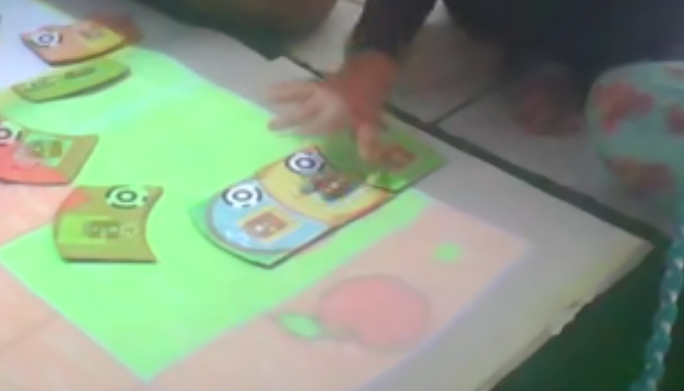
\includegraphics[width=.9\linewidth,fbox]{figs/percepcao_ra/mao_sobre_blocos.png}
        \caption{C11 coloca a mão sobre os blocos}
        \label{fig:mao_sobre_blocos}
    \end{subfigure}%
    \begin{subfigure}{.5\textwidth}
        \centering
        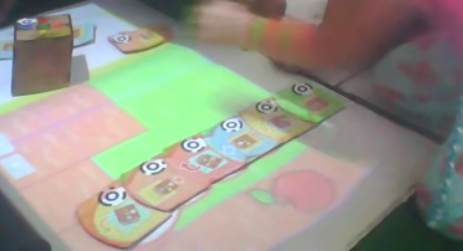
\includegraphics[width=.9\linewidth,fbox]{figs/percepcao_ra/sequencia_blocos.png}
        \caption{C10 encaixa blocos para ver a iluminação}
        \label{fig:sequencia_blocos}
    \end{subfigure}
    \caption{Exploração dos blocos}
    \label{fig:percepcoes_ra}
\end{figure}

Outros exemplos de interação com a RA foram tentativas de segurar a maçã ou tocar nos círculos de destaque dos blocos. A Equipe 5, por exemplo, percebeu o destaque dos blocos que aparece quando um algoritmo válido é criado. No primeiro momento em que a equipe, de modo exploratório, criou um algoritmo e a RoPE AR o destacou, C11 percebeu o destaque e aproximou a mão dos blocos (\autoref{fig:mao_sobre_blocos}). Em seguida, a colega C10 entendeu que o encaixe dos blocos provocou sua iluminação. Como consequência, C10 criou uma longa sequência de blocos, interessada em ver o efeito da iluminação sobre os mesmos  (\autoref{fig:sequencia_blocos}).

Essas ações indicam que a associação de elementos virtuais aos reais foi compreendida. Entretanto, essas ações ocorreram esporadicamente e as crianças rapidamente perderam o interesse ao perceber que os objetos virtuais não eram manipuláveis diretamente. As crianças também não demonstraram interesse pelo destaque, projetado em azul sobre blocos durante a execução. Em apenas três momentos houve apontamentos os círculos de destaque e nenhuma fala sobre eles. Esse recurso serviu como um auxílio para o pesquisador explicar a sequência de execução dos blocos, mas não eliminou a necessidade de apontá-los a mão.

Por fim, as crianças apresentaram interesse pela figura da maçã, que é uma entidade conhecida\footnote{Maçã é uma fruta presente nas refeições das crianças no CDI.}. Havia forte desejo de fazer o robô capturá-la. Para isso, as principais estratégias foram apertar os botões, mesmo que desativados, testar a combinação de diferentes blocos, e também empurrar o brinquedo com as mãos. O alcance do objetivo provocou reações de espanto e animação. Neste sentido, apesar de a tarefa ser repetitiva (sempre capturar a maçã), não se percebeu perda de engajamento. Pelo contrário, as crianças quiseram continuar a brincadeira mesmo após o término.

\section{Análise dedutiva}

A análise dedutiva teve como objetivo comparar as equipes e as atividades de programação e depuração. Ela segue a proposta de \citeonline{blikstein_analyzing_2014}, e inicia com uma definição prévia de códigos representando as ações das crianças. O \autoref{quadro:codigos} demonstra as ações mapeadas. Esses códigos foram analisados por dois pesquisadores de modo a obter um consenso sobre quais utilizar na etapa final de codificação. Ao obter consenso, o pesquisador codificou as etapas de programação e depuração captadas nos vídeos.

\begin{quadro}[!h]
    \begin{table_env}
    \caption{Ações mapeadas}
     \label{quadro:codigos}
     \begin{tabular}{@{}l m{.7\textwidth} c@{}}
        \toprule
        \textbf{Código} & \textbf{Descrição}  \\ \midrule
        Adiciona blocos & Aproxima dois ou mais blocos e os encaixa corretamente \\ \hline
        Adiciona bloco para resolver erro & Escolhe um bloco específico após a ocorrência de um erro \\ \hline
        Analisa robô & Manipula robô olhando para diversas partes dele \\ \hline
        Aperta botões & Aperta botões direcionais do brinquedo \\ \hline
        Aponta bloco & Aponta um bloco na lista de blocos \\ \hline
        Aponta bloco com erro & Aponta um bloco como a causa de um erro \\ \hline
        Aponta botão & Indica qual botão corresponde a uma ação \\ \hline
        Aponta caminho & Com a mão, mostra a direção que o RoPE deve seguir \\ \hline
        Aponta maçã & Indica a posição da maçã \\ \hline
        Aproxima bloco do robô & Aproxima um bloco do robô, com o intuito de que ele faça a ação do bloco \\ \hline
        Coloca brinquedo no início & Após erro, coloca brinquedo na posição inicial \\ \hline
        Coloca brinquedo sobre a maçã & Move diretamente o brinquedo para a posição final \\ \hline
        Usa comandos de voz & Fala a ação desejada para o RoPE \\ \hline
        Comemora & Apresenta sinais de alegria imediatamente após uma ação do brinquedo \\ \hline
        Cria hipótese & Sugere uma ação para solucionar um problema \\ \hline
        Distrai & Olha pros lados ou brinca com outros brinquedos da sala \\ \hline
        Escuta & Olha para o pesquisador ou professora enquanto eles falam \\ \hline
        Executa algoritmo com erro & Ciente do erro, mas inicia a execução para testar \\ \hline
        Executa passo & Aperta no botão que indica próxima ação do brinquedo, no modo de execução passo a passo \\ \hline
        Fala que comeu maçã & Percebe e fala que brinquedo capturou a maçã \\ \hline
        Fala sobre erro & Comenta sobre uma ação errada do RoPE \\ \hline
        Gira bloco & Gira um bloco para seta apontar em outra direção, mesmo que não encaixe na sequência de blocos \\ \hline
        Gira robô & Rotaciona brinquedo para que fique de frente para a maçã \\ \hline
        Inicia execução & Aperta botão Iniciar  \\ \hline
        Le algoritmo & Aponta, um por vez, os blocos encaixados em sequência \\ \hline
        Levanta robô procurando maçã & Após maçã sumir, levanta brinquedo do mapa \\ \hline
        Observa & Olha para blocos ou robô, sem tocar em nada \\ \hline
        Pensa com objeto na mão & Segura objeto, olha para ele e para o mapa \\ \hline
        Percebe que maçã apareceu & Aponta para maçã após ela aparecer \\ \hline
        Remove blocos & Retira um ou mais blocos de uma sequência de blocos encaixados \\ \hline
        Remove bloco com erro & Retira um ou mais blocos de uma sequência após a execução de um erro \\ \hline
        Reordena blocos & Muda a posição de um ou mais blocos na sequência de blocos \\ \hline
        Seleciona blocos & Procura um bloco para encaixar na sequência de blocos \\ \hline
        Simula passos do robô & Com a mão, move o RoPE e olha para os blocos \\ \hline
        Substitui bloco & Retira bloco e adiciona outro em seu lugar \\ \hline
        Substitui bloco com erro & Retira bloco e adiciona outro em seu lugar após um erro 
        \\ \bottomrule
        \end{tabular}
    \end{table_env}
    \sourceauthor
 \end{quadro}

 As ações foram então agrupadas em estados de alto nível (\autoref{quadro:estados}): entender, programar, depurar e executar. O estado Entender agrupa ações em que a criança busca informações para prosseguir a resolução da atividade, ou apresenta algum sinal de avaliação de um resultado. Programar agrupa ações de modificação do algoritmo do RoPE, seja por botões ou blocos. Depurar também abrange essas ações, mas quando ligadas a um erro recém-ocorrido. Por fim, o estado Executar se refere a iniciar execução e o estado Repousar significa apresentar sinais de distração.

 \begin{quadro}[!h]
    \begin{table_env}
    \caption{Estados}
     \label{quadro:estados}
     \begin{tabular}{@{}l m{.7\textwidth} c@{}}
        \toprule
        \textbf{Estados} & \textbf{Códigos}  \\ \midrule
        Entender & 

        \begin{itemize}
            \item Analisa robô
            \item Aponta bloco, botão, caminho ou maçã
            \item Coloca brinquedo sobre maçã
            \item Observa, olha blocos, olha robô
            \item Comemora, cria hipótese,
            \item Gira bloco ou robô
            \item Escuta
            \item Fala que "comeu"\ maçã, percebe que maçã apareceu
        \end{itemize} \\ \hline
        Programar & 

        \begin{itemize}
            \item Adiciona bloco, aperta botões
            \item Aproxima bloco do robo
            \item Comandos de voz
            \item Remove bloco
            \item Organiza blocos, reordena blocos, substitui bloco
            \item Seleciona blocos
        \end{itemize}
        \\ \hline
        Depurar & 

        \begin{itemize}
            \item Adiciona bloco resolvendo erro
            \item Aponta bloco com erro
            \item Coloca brinquedo no inicio após erro
            \item Executa algoritmo com erro
            \item Executa passo depuração
            \item Fala sobre erro
            \item Remove bloco com erro, substitui bloco com erro
        \end{itemize} 
        \\ \hline
        
        Executar &

        \begin{itemize}
            \item Inicia execução
        \end{itemize} 
        
        \\ \hline
        Repousar & 
        \begin{itemize}
            \item Se distrai
        \end{itemize} 

        \\ \bottomrule
        \end{tabular}
    \end{table_env}
    \sourceauthor
 \end{quadro}

A \autoref{fig:acoes_geral_programacao} demonstra o percentual de ações para todas as equipes nas fases de programação. Nessas fases a criança inicia construindo um algoritmo para resolver um problema, e podem ocorrer erros ou não. Nesse contexto, as ações mais frequentes foram entender (46.67\%), seguidas de programar (30.26\%) e executar (19.47\%). Ações relacionadas a depuração foram bem menos frequentes, com apenas 1.84\%. Por fim, apenas 1.75\% das ações estão relacionadas a repouso. Portanto, com maior frequência as crianças observaram e tentaram modificar os algoritmos, mas sem perceber ou corrigir erros. Também permaneceram focadas na tarefa. 

\begin{figure}[!htpb]
    \centering
    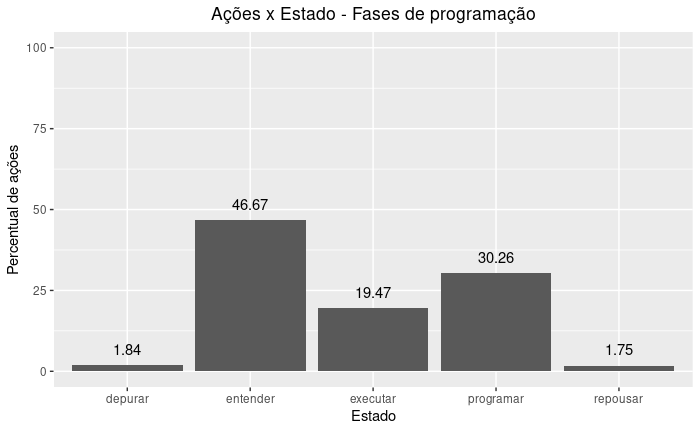
\includegraphics[width=.6\linewidth,fbox]{figs/graficos/acoes_geral_programacao.png}
    \caption{Percentual de ações em cada estado para todas as equipes, somente nas fases de programação.}
    \sourceauthor
    \label{fig:acoes_geral_programacao}
\end{figure}

A \autoref{fig:acoes_geral_depuracao} mostra o percentual de ações, em cada estado, somente nas etapas de depuração. O número de ações ligadas a depurar algoritmos aumenta para 15.58\%. Já as ações de entender e executar permanecem iguais aos níveis anteriores com margem de 2\%. As ações de programar diminuem para 16.3\%. Ocorreu, portanto, uma transferência do estado de programar para o estado de depurar. 

\begin{figure}[!htpb]
    \centering
    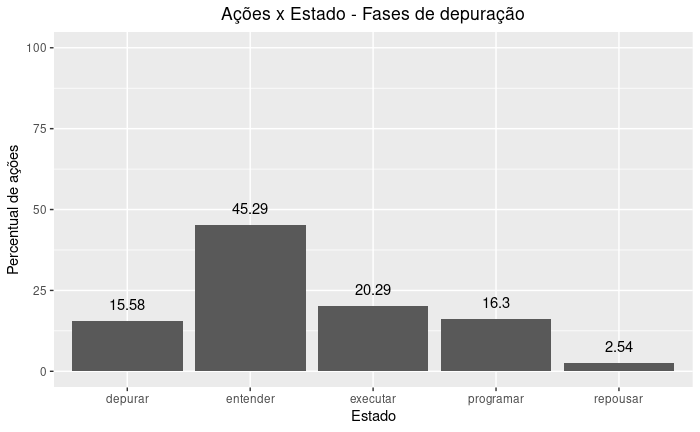
\includegraphics[width=.6\linewidth,fbox]{figs/graficos/acoes_geral_depuracao.png}
    \caption{Percentual de ações em cada estado para todas as equipes, nas fases de depuração}
    \sourceauthor
    \label{fig:acoes_geral_depuracao}
\end{figure}

 \subsection{Tempos por fase}

Além da codificação dos estados, também foram analisados os tempos despendidos por cada equipe em cada uma das 9 fases propostas. A obtenção dos tempos se deu por consultas SQL ao banco de dados armazenado pelo software Qualcoder. Após a extração, esses dados foram conferidos manualmente de modo a associar os tempos de cada fase às respectivas equipes. Por fim, a análise se deu utilizando a linguagem R no programa RStudio. Ressalta-se que não houve um critério pré-definido para a análise desses tempos. O objetivo foi explorar as diferenças e entre os tempos entre as equipes e entre as tarefas. 

 \begin{figure}[!htpb]
    \centering
    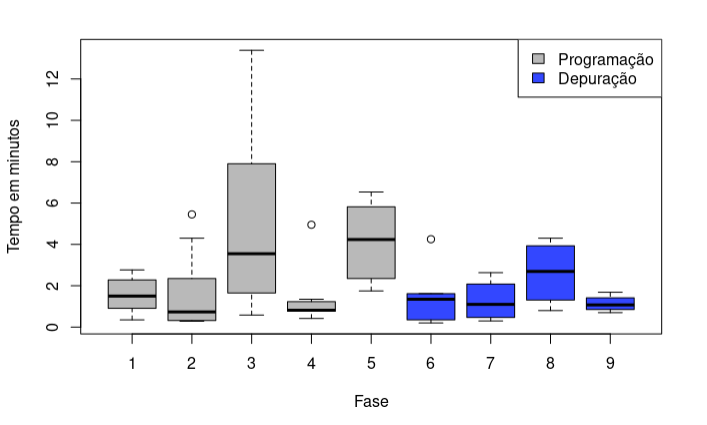
\includegraphics[width=.6\linewidth,fbox]{figs/tempos_por_tarefa.png}
    \caption{Distribuição de tempo por fases.}
    \sourceauthor
    \label{fig:tempo_tarefa}
\end{figure}

A \autoref{fig:tempo_tarefa} mostra os tempos de resolução de cada uma das 9 fases. Em cinza aparecem as 5 fases de programação, e em azul as 4 fases de depuração. Na etapa de programação, as fases 3 e 5 exigiram os maiores tempos de resolução. Uma possível causa para isso é que essas fases utilizam comandos de giro, que, conforme a literatura \cite{piaget_development_1964},  representa um obstáculo para as crianças. Destaca-se que a fase 3 é a primeira com comandos de giro, apresentou o maior tempo (mediana de 4 minutos).

A fase 7, de depuração, porém, é um contraponto. Ela também usa um comando de giro, sendo um espelho da fase 3. Enquanto uma usa os comandos Direita e Frente, a outra é solucionada por Esquerda e Frente. Teriam, portanto, a mesma complexidade. Apesar disso, a fase 7 foi resolvida em menos da metade do tempo da fase 3. Alguns fatores que podem influenciar nessa redução de tempo. É possível que a criança já tenha entendido como usar o comando de giro, pois precisou usá-lo anteriormente. Outra possibilidade é que, na fase de depuração os blocos já estão encaixados, e editar o algoritmo é mais fácil que construir um algoritmo sem nenhuma indicação inicial. A combinação desses dois fatores, compreensão do giro e edição mais fácil, também pode ter influenciado no resultado.

\section{Entrevistas}
As professoras responsáveis pelas turmas participantes foram entrevistadas após o término das atividades com as crianças. As questões aplicadas partiram de temas gerais, como a percepção do professor sobre o contato de crianças com tecnologias digitais (Q1), até a questão específica sobre a avaliação da RoPE AR (Q4). Aqui as respostas são apresentadas da temática mais específica para a mais geral.

Para a pergunta \pergunta{Q4 - Que problemas você percebe na proposta? Quais aspectos poderiam melhorar?}, as professoras consideraram não haver problemas perceptíveis na interface, ao menos do ponto de vista pedagógico.  Além disso, elas utilizaram adjetivos positivos para opinar sobre a RoPE AR:

    \citafalapessoa{Prof\_1}{Eu acho bem legal, porque é convidativo para eles assim. Isso poderia ser usado como se a gente colocasse um retroprojetor pra eles?}

    \citafalapessoa{Prof\_3}{[...] eu achei muito legal assim, porque eles gostaram assim, eles ficaram vidrados naquele robozinho. “E como é que comeu a maçã” eu achei engraçado né ele olhou por baixo onde é que vai a maçã né. Mas eu acho que ainda é um pouco distante.}

    \citafalapessoa{Prof\_4}{Isso é legal, isso é muito bom, gostei bastante. Eu achei que você ia colocar ali, como a gente tá acostumado né. Mas no chão foi muito legal...}

A Prof\_1 questiona se a aplicação poderia ser usada com o projetor na posição padrão, apontado para a parede. Isso indica incompreensão da proposta da interface, que é permitir a interação ativa das crianças para resolver problemas, ao invés de consumir conteúdo projetado na parede. A Prof\_4 também comenta que está acostumada ao uso do projetor, mas considera \fala{legal} o método de apontá-lo para o chão. Por fim, ela avalia a RoPE AR como um equipamento seguro:

    \citafalapessoa{Prof\_4}{Antes de tudo isso eu iria explicar pra eles que isso ali é um projetor, que teriam que cuidar pra não bater, porque também a gente trabalha com projetor na parede né, então quando a gente traz a gente diz que só a prof pode mexer, eles não podem mexer. [...] Eu não vejo como um perigo para eles. Isso não ia cair em cima de uma criança e machucar. No máximo iria quebrar, no máximo teria um prejuízo. A gente se preocupa mais se fosse uma coisa muito pesada e poderia machucar uma criança.}

A Prof\_3 avalia positivamente a RoPE AR, mas acha que é uma realidade \fala{distante} devido ao custo de implementar um espaço exclusivo para equipamentos \fala{caros} e à ausência de \fala{formação tecnológica} para os professores.

    \citafalapessoa{Prof\_3}{Mas eu acho que ainda é um pouco distante. Talvez daqui mais algum tempo, quando isso ficar mais acessível. Porque eu sei que um laboratório, informática e tudo, digital, isso é um investimento alto né, então fica mais nas universidades. [...] Porque nós professores, nós não temos a formação tecnológica né. }

Quanto às aplicações da RoPE AR (Q3), a Prof\_3 sugere a construção de jogos de tabuleiro, e a exploração musical para discriminação auditiva. A proposta é emitir o som do instrumento quando o RoPE chegar sobre ele. No mesmo sentido, a professora também sugere emitir o som de letras.

\citafalapessoa{Prof\_3}{
    Poderia até fazer jogos de tabuleiro. Dependendo onde você vai, tem que avançar na casa, retroceder, voltar no jogo... que é interessante também né pros menores, porque eles gostam bastante. Tem jogos mais simples, jogos mais complexos. Tipo um caça palavras ali, pras crianças que são alfabetizadas seria interessante. [...] Ou ele faz um som e aparece... vamos supor, se for um instrumento musical, se aparece um som daquilo ele pode estar identificando, por exemplo, deu um som de trovão, tem a figura do trovão e ele vai ter que associar. É um outro jogo no mesmo [estilo], mas com outra função, que eu posso associar. Porque quem tá fazendo associação de sons, né, discriminação auditivia, brincadeiras de discriminação auditivia, ele pode chegar em determinado local, fazer um som, e daquilo a criança vai ter que identificar qual é pra seguir adiante. Ou até uma letra. Ele chega até uma letra, ele faz o som.
}

Já a Prof\_4 sugere utilizar o princípio da detecção de posição do RoPE para contação de histórias. A interface poderia projetar um lobo,  o qual o RoPE deveria seguir.

\citafalapessoa{Prof\_4}{
    É, tipo se fosse uma contação de história? Vai contando uma história e o robô vai demonstrando um cenário, vai chegando perto do cenário e vai fazendo um personagem da história. Eu pensaria nisso... Tipo um lobo, chegou no mato e o robô segue o lobo, algo assim, e vai chegando...
}

Para a Q2 - \pergunta{Que importância você daria para a \destaque{visibilidade} no aprendizado das crianças?}, todas as professoras afirmaram ser necessário o contato com materiais concretos.

    \citafalapessoa{Prof\_1}{Ah, eu acho importantíssimo, porque eu sou visual, eu aprendo muito mais olhando e ouvindo, presencial. Tirar dúvidas né, na hora... [...] tem que mostrar, aprende muito mais. }

    \citafalapessoa{Prof\_3}{ Ah, sim. Pros menores, até a criança de sete, oito anos, é sempre concreto né, é sempre a partir daquele material, que ele possa pegar, visualizar, pra ele internalizar. Porque o abstrato assim, ficar explicando muito, eles não vão conseguir fazer a associação. Eles precisam associar que uma coisa é ligada a outra. Então eles têm que pegar, eles têm que sentir, eles têm que ver. Essa forma ali, eles conseguiram ter os comandos na hora.}

A Prof\_3 ainda comenta, a partir de uma observação do pesquisador, a respeito de toquinhos de madeira que estavam presentes na sala. Segundo ela, materiais não-estruturados são imprescindíveis nos espaços educacionais:

    \citafalapessoa{Prof\_3}{A gente está acostumado com plástico. Então plástico, madeira, são outras possibilidades de construção. Esses dias ele [uma criança] tava fazendo um prédio, disse que tava fazendo um prédio. Ele empilhou todos os toquinhos assim. Então é isso mesmo, é construir ou construir uma cerca. O bloco é essa tentativa. Ele não é um objeto muito estruturado. A criança tem que ter contato com objetos não estruturados. Então ele não tem forma, ele não deve para um devido fim. Ele vai montar uma estrutura a partir daquele objeto que não tem formato. Ele que vai ter que imaginar e dar forma àquele objeto. Então o objeto não estruturado é imprescindível que tenha no espaço de educação. }

Os blocos de código, assim como os toquinhos de madeira, também são elementos não estruturados. A criança os organiza para definir uma rota, uma história, ou um comportamento para o brinquedo RoPE. Neste sentido, os materiais do ambiente visitado e a proposta da pesquisa se assemelham: são objetos concretos e não estruturados, que a criança estrutura conforme seu desejo.

Por fim, a questão mais geral (Q1): \pergunta{O que você pensa sobre o contato de crianças com tecnologias digitais?} teve as respostas a seguir:

    \citafalapessoa{Prof\_1}{[...] é uma forma educativa de inserir eles na informatização, porque em casa o celular e a tecnologia é só voltada pro YouTube, coisas que não são tão úteis. E se a gente puder introduzir isso de uma forma que eles procurem no Google o conhecimento, informática... isso é bem legal. Interessante. Mudar o foco do YouTube...}

    \citafalapessoa{Prof\_3}{Eu acho fantástico, é uma pena que nós não temos né. Na rede pública é mais difícil porque ter mais equipamentos né, de pesquisa com as crianças, como uma mesa digital, isso é muito custoso né, pro município ter.}

    \citafalapessoa{Prof\_4}{Ah, eu acho necessário. Eu acho necessário, mas também tem que ter o equilíbrio assim. Tu não pode deixar a criança só com tecnologia, vamos supor, o celular, que é o que eles tem em mãos, né, que a gente viu que foi o que aconteceu com alguns, que passaram a pandemia toda com o celular na mão, tem que ter o equilíbrio.}

As respostas da Q1 evidenciam a percepção negativa sobre o acesso exagerado, não supervisionado e passivo das crianças a equipamentos eletrônicos para assistir vídeos na internet. A Prof\_1 cita a necessidade de \fala{mudar o foco do YouTube}, e a Prof\_4 fala que não se \fala{pode deixar a criança ‘só’ com a tecnologia}. 

As respostas evidenciam uma percepção positiva da RoPE AR. As sugestões de aplicações da interface incluíram jogos de tabuleiro, atividades para reconhecer letras e sons, e também contação de histórias. Uma conclusão é que as professoras perceberam potencial pedagógico no uso do princípio de aplicar realidade aumentada associada a objetos concretos, à captação de posições desses objetos, e à emissão de sons. O suporte a essas aplicações, entretanto, exigiria uma plataforma de configuração, como o exemplo da Ct Puzzle Platform, mas que foge do foco da atual pesquisa. 

As professoras não tiveram contato com a etapa de instalação e conexão dos equipamentos. Essa etapa apresentou dificuldades de conexão em uma das salas, conforme relatado na descrição do contexto de pesquisa. É possível que apresentassem uma opinião menos positiva a respeito da interface em caso de a usarem por conta própria.